%%%%%%%%%%%%%%%%%%%%%%%%%%%%%%%%%%%%%%%%%%%%%%%%%%%%%%%%%%%%%%%%%%%%%%%%%%%
%
% Generic template for TFC/TFM/TFG/Tesis
%
% $Id: estudioTeorico.tex,v 1.5 2015/06/05 00:05:19 macias Exp $
%
% By:
%  + Javier Macías-Guarasa.
%    Departamento de Electrónica
%    Universidad de Alcalá
%  + Roberto Barra-Chicote.
%    Departamento de Ingeniería Electrónica
%    Universidad Politécnica de Madrid
% 
% Based on original sources by Roberto Barra, Manuel Ocaña, Jesús Nuevo, Pedro Revenga, Fernando Herránz and Noelia Hernández. Thanks a lot to all of them, and to the many anonymous contributors found (thanks to google) that provided help in setting all this up.
%
% See also the additionalContributors.txt file to check the name of additional contributors to this work.
%
% If you think you can add pieces of relevant/useful examples, improvements, please contact us at (macias@depeca.uah.es)
%
% You can freely use this template and please contribute with comments or suggestions!!!
%
%%%%%%%%%%%%%%%%%%%%%%%%%%%%%%%%%%%%%%%%%%%%%%%%%%%%%%%%%%%%%%%%%%%%%%%%%%%

\chapter{Estado del arte}\label{cha:estado-arte}

En este capítulo, se lleva a cabo la explicación de distintos aspectos teóricos esenciales para el entendimiento del desarrollo del proyecto.
Para ello, este capítulo se dividirá en dos apartados principales: criptografía e \ac{IoT}.


\section{Criptografía}\label{sec:criptografia}

En este primer apartado se van a mostrar distintos aspectos importantes en lo referente a la criptografía, como pueden ser las características principales así como los esquemas utilizados actualmente, el paradigma de la computación cuántica y la criptografía postcuántica.


\subsection{Características}\label{subsec:caracteristicas}

La criptografía consiste en el cifrado de datos con el objetivo de obtener confidencialidad e integridad.
Para ello, a lo largo de la historia se han utilizado distintos esquemas, como pueden ser el cifrado César, el cual se basa en la sustitución de los caracteres utilizados por los caracteres a una determinada cantidad de posiciones dentro del abecedario.
Otro esquema utilizado es el sistema Vigenère, el cual se basa en desplazamiento, en el cual cada caracter se desplaza una cantidad de posiciones independiente, de forma que se genera un vector k (número de posiciones desplazadas de cada caracter) que representa la clave para el sistema.

En los sistemas criptográficos se pueden buscar 4 posibles tipos de seguridad:

\begin{itemize}
    \item \textbf{Seguridad incondicional}: El sistema es seguro, sin importar los recursos de los que disponga el atacante.
    \item \textbf{Seguridad computacional}: El sistema es seguro frente a un atacante con recursos computacionales limitados
    \item \textbf{Seguridad heurística}: No se ha demostrado seguro pero, por el momento, no se ha enccontrado forma de romper el sistema.
    \item \textbf{Seguridad condicional}: Cualquier sistema que no se incluye en las categorías anteriores.
\end{itemize}

Los sistemas actuales se basan en la seguridad computacional, por lo que, ante el avance en la capacidad de computación, estos se deben actualizar para mantener la seguridad deseada.

Dentro de estos sistemas, se pueden diferenciar dos tipos: los sistemas de clave simétrica y los sistemas de clave asimétrica.
Estos primeros utilizan una única clave en ambos extremos de la comunicación, de forma que ambos usuarios utilizan la misma clave para cifrar y descifrar.
Los sistemas de clave asimétrica hacen uso de dos claves distintas: una pública y otra privada.
La clave pública es conocida por todos los usuarios y se puede utilizar para cifrar un mensaje cuyo destinatario sea el propietario de esas claves.
La clave privada solamente es conocida por el usuario que la crea y se utiliza para descifrar un mensaje cifrado con la clave pública.
Además, se puede utilizar la clave privada para firmar un mensaje y, dicha firma, se puede verificar mediante el uso de la clave pública.


\subsection{Modelos actuales}\label{subsec:mod_act}

En cuanto a los sistemas de clave asimétrica actuales, es necesario mencionar RSA, DSA y sistemas basados en curva elíptica.


\subsubsection{RSA}\label{subsubsec:rsa}

El mecanismo RSA se desarrolló en 1979 y su seguridad se basa en la factorización de números enteros.

En cuanto al funcionamiento del mecanismo, en primer lugar, se generan las claves, para lo cual se han de elegir dos números primos disntintos (\textit{p} y \textit{q}) de forma aleatorio en de longitud en bits similar.
Con el producto de estos dos números se obtiene el módulo para ambas claves \textit{n}.
A continuación, se escoge el exponente de la clave pública \textit{e} y un respectivo exponente de la clave privada \textit{d}, de forma que cumplan $e\times d\equiv 1$.
De esta forma, es posible cifrar un texto \textit{m} mediante $m^{e} (mod n)$.
Para descifrar dicho texto cifrado, se debe ejecutar $c^{d} (mod n)$.

Desde el año 2002, se recomendó que las claves fueran de, al menos, 1024 bits aunque, en 2015, el \ac{NIST} consideró que la longitud mínima de las claves debe ser de, por lo menos, 2048 bits.
Por el momento, existe un gran debate acerca de si la computación cuántica será capaz de resolver el problema en el que se basa este algoritmo en poco tiempo de ejecución, inutilizando así este algoritmo incluso con tamaños de clave mayores.


\subsubsection{DSA}\label{subsubsec:dsa}

Por otro lado, tenemos el algoritmo de firma DSA, el cuál se desarrolló en el año 1991.
Este algoritmo fue propuesto por el \ac{NIST} en su \ac{DSS}.

Este mecanismo dispone de 3 funciones distintas: generación de claves, firma y verificación.
Para la generación de claves, se debe elegir un número primo \textit{p} cuya longitud en bits sea divisible por 64.
A continuación, se debe escoger un número primo \textit{q} de 160 bits tal que $p-1=qz$ donde z es un número natural.
También, se debe elegir \textit{h} de forma que $1 < h < p-1$ y $h^z (mod p) > 1$ y \textit{x} de forma que $1 < x < q-1$.
Por último, se computa $y=g^x(mod p)$.
Los datos públicos son \textit{p}, \textit{q}, \textit{g} e \textit{y}.
La clave privada es \textit{x}.

Para la firma, se debe escoger un número aleatorio \textit{k} de forma que $1 < k < q$.
A continuación, se calcula $r = (g^k mod p) mod q$ y $s = k^{-1} (H(m) + r\times x) mod q$, donde H(m) es una función resumen sobre el mensaje m.
La firma del mensaje es el par (r,s).

En cuanto a la verificación, se debe calcular $w = s^{-1} mod q$, $u_1 = (H(m)\times w) mod q$, $u_2 = (r\times w) mod q$ y $v = [g^{u_1}\times y^{u_2} mod p] mod q$.
Si se cumple $v = r$, la firma es correcta.

Respecto a este algoritmo, el \ac{NIST} ha recomendado el uso de claves de, como poco, 2048 bits y no recomienda el uso de la función resumen SHA-1.


\subsubsection{Curva elíptica}\label{subsubsec:eliptica}

Por último, se hace uso de sistemas que emplean curva elíptica ya que estos proporcionan una seguridad equivalente en una longitud de clave menor.

Una curva elíptica se representa mediante la ecuación $y^2 = x^3 + ax + b$.
Para su uso en criptografía, se utiliza un punto base G publicado con un curva específica.
A continuación, se escoge un número entero aleatorio \textit{k}, el cual se utiliza como clave privada.
La clave pública se genera mediante el producto $P = k\times G$.


\subsection{Computación cuántica}\label{subsec:cuantica}

La computación cuántica supone avance tecnológico en cuanto a capacidad de cálculo respecto a los actuales computadores.
Este tipo de computación se basa en el uso de los denominados bits cuánticos (o qubits), sustituyendo así los bits utilizados en la computación clásica.
Estos qubits se explotan mediante diversas características de la mecánica cuántica como la superposición, la interferencia o su entrelazamiento~\cite{Rietsche2022}.

\begin{figure}[h]
    \centering
    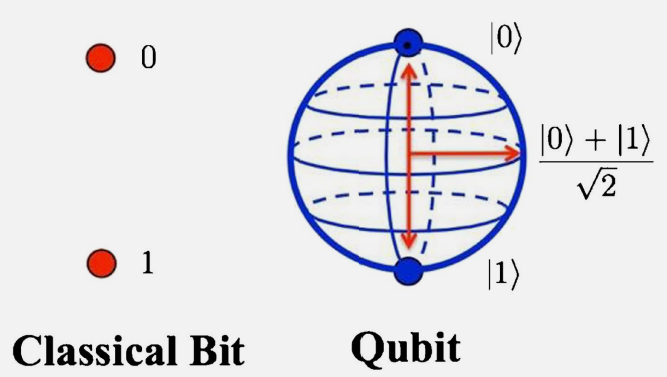
\includegraphics[width=0.6\textwidth]{figures/qubit.png}
    \caption{Bit clásico y qubit~\cite{Rietsche2022}.}
    \label{fig:qubit}
\end{figure}

La forma de trabajar con estos qubits consiste en la consideración de la probabilidad de los bits de encontrarse en un valor o en otro, es decir, siguiendo la Fórmula~\ref{eqn:quantum}.

\begin{equation}\label{eqn:quantum}
    \sum_{b\in {\{0, 1\}}^n} p_b \ket{b}
\end{equation}

A la hora de conocer con exactitud el valor de dicho qubit,es importante mencionar que, al medir su valor, dicho qubit colapsa a uno de los valores tradicionales (``0'' o ``1'').
Teniendo en cuenta la propiedad de superposición de estos qubits, un computador cuántico es capaz de representar 16 números de 4 dígitos cada uno utilizando, únicamente, 4 qubits.
Por ello, estos dispositivos pueden realizar una cantidad exponencial de cálculos a la vez.
También, gracias al entrelazamiento cuántico, los qubits se encuentran relacionados unos con otros, de forma que el estado de cada qubit puede depender de otro qubit.
De esta forma, se consigue una correlación entre qubits no existente en los bits convencionales.

Respecto a la capa \textit{software}, esta debe lidiar con el ruido térmico que puede afectar al funcionamiento de estos computadores.
Para evitar el impacto de este ruido, algunos computadores cuánticos deben ser utilizados a menos de una centésima de grado por encima del cero absoluto.

Esta tecnología está siendo ampliamente investigada y desarrollada con el objetivo de conseguir un mayor número de qubits funcionales y, por ende, una mayor capacidad de computación.
En la Figura~\ref{fig:progress-qubits} se representa el aumento en número de qubits de los computadores cuánticos con el avance de los años.

\begin{figure}[h]
    \centering
    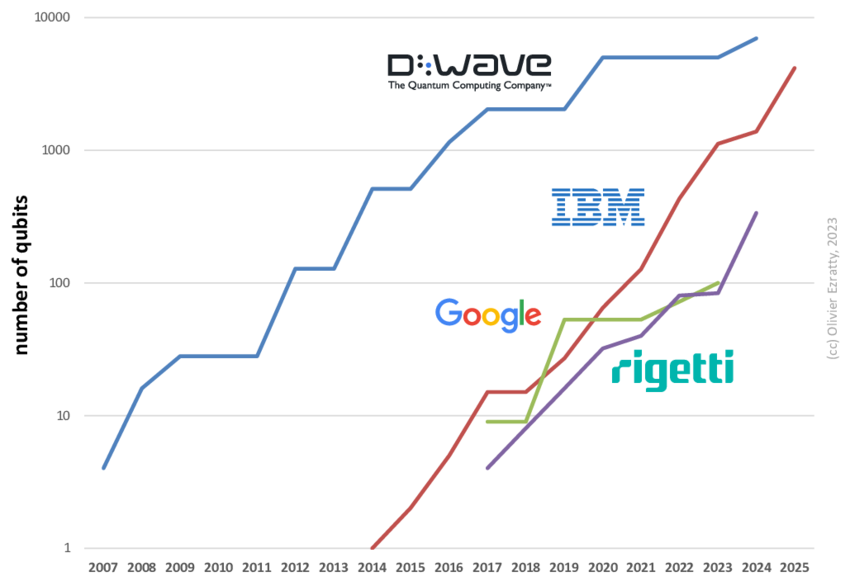
\includegraphics[width=0.85\textwidth]{figures/progress-qubits.png}
    \caption{Progreso en el número de qubits de un computador cuántico~\cite{progress-qubits}.}
    \label{fig:progress-qubits}
\end{figure}

Gracias a este progreso en el número de los qubits disponibles en los computadores cuánticos, estos consiguen una capacidad de cómputo muy superior a los ordenadores convencionales.


\subsection{Criptografía postcuántica}\label{subsec:postcuantica}

Debido a este incremento en las capacidades de los computadores cuánticos y el hecho de que los sistemas criptográficos actuales se basan en seguridad computacional, es necesario asegurar la privacidad de los usuarios.
Para ello, se ha optado por sustituir los esquemas actuales de clave pública por otros capaces de asegurar la privacidad de los usuarios frente a este nuevo paradigma.

Los nuevos algoritmos diseñados se pueden dividir en dos tipos:

\begin{itemize}
    \item \textbf{Signature}: Este tipo de algoritmos lleva a cabo la firma de una cadena mediante el uso de claves asimétricas.
    \item \textbf{\ac{KEM}}: Este tipo de mecanismo lleva a cabo la compartición de un secreto únicamente conocido por los dos extremos de la comunicación.
\end{itemize}

El mecanismo de firma (\textit{Signature}), hace uso de tres funciones:

\begin{itemize}
    \item Generación de claves.
    \item Firma de la cadena.
    \item Verificación de la firma.
\end{itemize}

En la generación de las claves, se crean tanto la clave pública como la clave privada.
En la firma de la cadena, se utiliza la clave privada para indicar a los receptores del mensaje que este ha sido enviado por el emisor indicado de forma inequívoca.
Por último, se utiliza la verificación de la firma para comprobar que el emisor indicado es correcto y la integridad del mensaje.

El mecanismo \ac{KEM} hace uso de otras tres funciones:

\begin{itemize}
    \item Generación de claves.
    \item Encapsulado.
    \item Desencapsulado.
\end{itemize}

En la generación de las claves, se crean tanto la clave pública como la clave privada.
En la función de encapsulado genera el secreto compartido y un texto cifrado.
En la función de desencapsulado, se utiliza el texto cifrado anteriormente creado para obtener el secreto compartido.
De esta forma, ambos usuarios disponen del secreto compartido sin haberlo intercambiado directamente.



\subsubsection{Dilithium}\label{subsubsec:dilithium}

Dilithium~\cite{dilithium} es un algoritmo criptográfico de firma digital basado en retículos.
Este algoritmo fue seleccionado por el \ac{NIST} como estándar para un sistema de firma postcuántica~\cite{nist_sel}.

El esquema Dilithium se basa en Fiat-Shamir con abortos~\cite{10.1007/978-3-642-10366-7_35} y consta de tres funciones principales: una función de generación de claves, una función de firma y una función de comprobación de firma~\cite{dilithium_spec}.
En cuanto a la generación de las claves, se proporciona el Algoritmo~\ref{alg:gen_dilithium}.
En este proceso, se genera una matriz A de dimensiones $k \times l$ y, posteriormente, se obtienen vectores aleatorios de la clave secreta.

\begin{algorithm}
    \caption{Generación de claves pública y privadas en Dilithium~\cite{dilithium_spec}.}
    \label{alg:gen_dilithium}
    %\KwData{Nada}
    \KwResult{Claves pública y privada.}
    \hspace{2mm}$\textbf{A} \gets R_q^{k\times l}$\newline
    $(s_1,s_2) \gets S_\eta^l \times S_\eta^{k}$\newline
    $\textbf{t} := \textbf{A}s_1 + s_2$\newline
    \textbf{return} (pk = (\textbf{A}, \textbf{t}), sk = (\textbf{A}, \textbf{t}, $s_1$, $s_2$))
\end{algorithm}

En lo respectivo a la firma, esta se muestra en el algoritmo~\ref{alg:sign_dilithium}.
En él, se genera un vector de enmascaramiento de polinomios \textbf{y} con coeficientes menores que $\gamma_1$.
El parámetro $\gamma_1$ se escoge de forma que sea lo suficientemente grande como para no revelar la clave secreta pero no demasiado grande como para que la firma sea fácilmente falsificable.
A continuación, establece $w_1$ como los bits de mayor orden del cómputo \textbf{Ay} y obtiene c como la función resumen del mensaje y $w_1$.
Para evitar que \textbf{z} filtre la clave privada, se lleva a cabo una comprobación de que los componentes de \textbf{z} son menores que $\gamma_1 - \beta$.
En caso contrario, se reinicia el procedimiento.

\begin{algorithm}
    \caption{Firma en Dilithium~\cite{dilithium_spec}.}
    \label{alg:sign_dilithium}
    \KwData{Clave privada y mensaje a firmar.}
    \KwResult{Firma digital.}
    \hspace{2mm}$\textbf{z} := \perp$\newline
    \While{$z = \perp$}{
        \hspace{2mm}$y \gets S_{\gamma 1-1}^l$\newline
        $w_1 := HighBits(\textbf{Ay}, 2\gamma_2)$\newline
        $c\in B_\tau := H(M||w_1)$\newline
        $\textbf{z} := \textbf{y} + cs_1$\newline
        \If{$||z||_{\infty}\geq \gamma_1-\beta$ or $||LowBits(\textbf{Ay} - cs_2, 2\gamma_2)||_\infty\geq \gamma_2 - \beta$}{
            $\textbf{z} := \perp$
        }
    }
    \textbf{return} $\sigma = (\textbf{z}, c)$
\end{algorithm}

Finalmente, para el sistema de verificación de firma, se dispone del algoritmo~\ref{alg:ver_dilithium}.
En esta función, se computa ${w'}_1$ como los bits de mayor orden de \textbf{Az}-ct y acepta si todos los coeficientes de \textbf{z} menores que $\gamma_1 - \beta$ y si c es el resultado de la función resumen del mensaje y ${w'}_1$.

\begin{algorithm}
    \caption{Verificación de firma en Dilithium~\cite{dilithium_spec}.}
    \label{alg:ver_dilithium}
    \KwData{Clave pública y mensaje firmado.}
    \KwResult{Mensaje original.}
    \hspace{2mm}${w'}_1 := HighBits(\textbf{Ay}, 2\gamma_2)$\newline
    \If{$[||\textbf{z}||_\infty < \gamma_1 - \beta]$ \textbf{and} $[c = H(M||{w'}_1)]$}{
        \textbf{return}
    }
\end{algorithm}

Los algoritmos~\ref{alg:gen_dilithium},~\ref{alg:sign_dilithium} y~\ref{alg:ver_dilithium} son la versión simplificada pero menos eficiente del algoritmo.
Se ha decidido explicar brevemente estos diseños para otorgar un conocimiento aceptable pero no total ya que, con el entendimiento de dichos algoritmos, es suficiente.

Dilithium consta de tres versiones: Dilithium2, Dilithium3 y Dilithium5.
La diferencia entre estas consiste en el tamaño de las claves y firmas generadas.
En la tabla~\ref{tab:dilithium} se muestran los distintos tamaos a tener en cuenta de cada versión del algoritmo.
Además, se indica la seguridad ante el ataque Quantum Core-SVP tanto con \ac{SIS} como con \ac{LWE}.

\begin{table}[H]
    \centering
    \begin{tabular}{|c|c|c|c|}
    \hline
                                & \textbf{Dilithium2}   & \textbf{Dilithium3}   & \textbf{Dilithium5}   \\ \hline
    Clave pública (bytes)       & 1312                  & 1952                  & 2592                  \\ \hline
    Clave privada (bytes)       & 2528                  & 4000                  & 4864                  \\ \hline
    Firma (bytes)               & 2420                  & 3293                  & 4595                  \\ \hline
    Seguridad ante LWE (bits)   & 112                   & 165                   & 229                   \\ \hline
    Seguridad ante SIS (bits)   & 112                   & 169                   & 241                   \\ \hline
    \end{tabular}
    \caption{Diferencias entre versiones de Dilithium~\cite{dilithium_spec}.}
    \label{tab:dilithium}
\end{table}



\subsubsection{Kyber}\label{subsubsec:kyber}


\begin{algorithm}
    \caption{Generación de claves en Kyber~\cite{kyber_spec}.}
    \label{alg:gen_kyber}
    %\KwData{}
    \KwResult{Claves pública y privada.}
    \hspace{2mm}$d \gets B^{32}$\newline
    $\rho\sigma := G(d)$\newline
    $N := 0$\newline
    \For{i from 0 to k-1}{
        \For{j from 0 to k-1}{
            Â$[i][j] := Parse(XOF(\rho, j, i))$
        }
    }
    \For{i from 0 to k-1}{
        $s[i] := CBD_{\eta 1}(PRF(\sigma, N))$\newline
        N := N + 1
    }
    \For{i from 0 to k-1}{
        $e[i] := CBD_{\eta 1}(PRF(\sigma, N))$\newline
        N := N + 1
    }
    %$a$\newline
\end{algorithm}


\begin{table}[H]
    \centering
    \begin{tabular}{|c|c|c|c|}
    \hline
                                & \textbf{Kyber512}     & \textbf{Kyber768}    & \textbf{Kyber1024}   \\ \hline
    Clave pública (bytes)       & 800                   & 1184                 & 1568                 \\ \hline
    Clave privada (bytes)       & 1632                  & 2400                 & 3168                 \\ \hline
    Texto cifrado (bytes)       & 768                   & 1088                 & 1568                 \\ \hline
    Secreto compartido (bytes)  & 32                    & 32                   & 64                   \\ \hline
    Core-SVP Quantum Hardness (bits)& 107                    & 165                   & 232                   \\ \hline
    \end{tabular}
    \caption{Diferencias entre versiones de Kyber~\cite{kyber_spec}.}
    \label{tab:kyber}
\end{table}

\subsubsection{Sphincs+}\label{subsubsec:sphincs}

Sphincs+ es un algoritmo de firma basado en un esquema de firma única diseñado por Lamport~\cite{lamport1979constructing} en la década de 1970, el cual fue mejorado para desarrollar el sisteam XMSS.
Este algoritmo fue elegido por el \ac{NIST} como estándar en algoritmos de firma.

Sphincs+ dispone de gran cantidad de variables, a diferencia del resto de algoritmos.
En este algoritmo, ofrece una elección entre optimización para tamaño (terminación ``s'') u optimización para velocidad (terminaación ``f'').
Además, permite elegir entre una implementación simple (sin considerar máscaras) o robusta (considerando máscaras).
Por último, permite la elección entre el uso de distintas funciones resumen: SHA2, SHAKE o Haraka.
En la tabla~\ref{tab:sphincs} se puede comprobar los tamaños de los distintos elementos que componen este algoritmo.

\begin{table}[H]
    \centering
    \begin{tabular}{|c|c|c|c|}
    \hline
                            & Clave pública (bytes) & Clave privada (bytes) & Firma (bytes) \\ \hline
    \textbf{Sphincs-128s}   & 32                    & 64                    & 7856          \\ \hline
    \textbf{Sphincs-128f}   & 32                    & 64                    & 17088         \\ \hline
    \textbf{Sphincs-192s}   & 48                    & 96                    & 16224         \\ \hline
    \textbf{Sphincs-192f}   & 48                    & 96                    & 35664         \\ \hline
    \textbf{Sphincs-256s}   & 64                    & 128                   & 29792         \\ \hline
    \textbf{Sphincs-256f}   & 64                    & 128                   & 49856         \\ \hline
    \end{tabular}
    \caption{Tamaños de las diferentes versiones de Sphincs+~\cite{sphincs_spec}.}
    \label{tab:sphincs}
\end{table}


\subsubsection{McEliece}\label{subsubsec:mceliece}

El algoritmo McEliece se trata de un algoritmo \ac{KEM} que fue diseñado para resistir \ac{OW-CPA}, de forma que un atacante no puede obtener de forma eficiente la clave privada partiendo de un texto cifrado y la clave pública.
Este algoritmo ha mantenido una seguridad considerablemente estable pese a los muchos ataques intentados.
Inicialmente, se diseñó para obtener 64 bits de seguridad, aunque este factor escala fácilmente para estar al día con los avances en la computación.

Algunos de los parámetros importantes en este algoritmo son \textit{n} como la longitud de código y \textit{k} como dimensión de código, ambos especificados de acuerdo a la versión del algoritmo.

Para la generación de las claves pública y privada se lleva a cabo el siguiente proceso~\cite{mceliece_spec}:

\begin{enumerate}
    \item Se genera una cadena aleatoria y uniforme \textit{s} con longitud \textit{n} bits.
    \item Se genera un polinomio aleatorio, uniforme e irreducible $g(x)\in F_q[x]$ de grado \textit{t}.
    \item Se genera una secuencia aleatoria y uniforme ($\alpha_1, \alpha_2,...,\alpha_n$) con \textit{n} elementos distintos de $F_q$.
    \item Se define $\Gamma =(g,\alpha_1, \alpha_2,...,\alpha_n)$.
    \item Se ejecuta $MatGen(\Gamma)=(T,c_{n-k-\mu+1},...,c_{n-k},\Gamma')$ donde MatGen es una función propia del algoritmo para la generación de una matriz.
    \item La clave pública está representada por \textit{T} mientras que la clave privada se compone por ($\Gamma',s$).
\end{enumerate}

En cuanto a la generación del encapsulado, se deben llevar a cabo los siguientes pasos~\cite{mceliece_spec}:

\begin{enumerate}
    \item Se genera un vector aleatorio y uniforme $e\in F_2^n$ de peso \textit{t}.
    \item Se define $H=(I_{n-k}|T)$ y se computa $C_0=He\in F_2^{n-k}$.
    \item Se calcula $C_1=H(2,e)$, donde H representa una función resumen.
    \item Se computa $K=H(1,e,C)$.
    \item Se obtiene el texto cifrado \textit{C} y el secreto compartido \textit{K}.
\end{enumerate}

Respecto al desencapsulado, se llevan a cabo las siguientes operaciones~\cite{mceliece_spec}:

\begin{enumerate}
    \item Se separa el texto cifrado \textit{C} en ($C_0,C_1$) con $C_0\in F_2^{n-k}$ y $C_1\in F_2^l$.
    \item Se asigna $b\leftarrow 1$.
    \item Se extraen $s\in F_2^n$ y $\Gamma'=(g,\alpha'_1, \alpha'_2,...,\alpha'_n)$ de la clave privada.
    \item Se extiende $C_0$ a $v=(C_0,0,...,0)\in F_2^n$ y se busca la única clave \textit{c} definida por $\Gamma'$ que se encuentra a menor distancia \textit{t} de $v$.
    \item Se asigna $e=v+c$ y, si no se cumple que $wt(e)=\textit{t}$ y $C_0=He$, $e\leftarrow \perp$
    \item Si $e=\perp$, $e\leftarrow s$ y $b\leftarrow 0$.
    \item Se calcula $C'_1=H(2,e)$ donde H es una función resumen.
    \item Si $C'_1\neq C_1$, $e\leftarrow s$ y $b\leftarrow 0$.
    \item Se otiene $K=H(b,e,C)$, donde K es el secreto compartido.
\end{enumerate}

Este algoritmo emplea varias versiones, cada una con distintas longitudes de clave y textos cifrados.
Estas diferencias se muestran en la Tabla~\ref{tab:mceliece}. 

\begin{table}[H]
    \centering
    \begin{tabular}{|c|c|c|c|c|c|}
    \hline
    Versiones                   & \textbf{348864}  & \textbf{460896}  & \textbf{6688128} & \textbf{6960119} & \textbf{8192128} \\ \hline
    Clave pública (bytes)       & 261120                    & 524160                    & 1044992                   & 1047319                   & 1357824                   \\ \hline
    Clave privada (bytes)       & 6492                      & 13068                     & 13932                     & 13948                     & 14120                     \\ \hline
    Texto cifrado (bytes)       & 96                        & 156                       & 208                       & 194                       & 208                       \\ \hline
    Secreto compartido (bytes)  & 32                        & 32                        & 32                        & 32                        & 32                        \\ \hline
    \end{tabular}
    \caption{Diferencias entre versiones de McEliece~\cite{mceliece_spec}.}
    \label{tab:mceliece}
\end{table}


\subsubsection{HQC}\label{subsubsec:hqc}

El algoritmo HQC es un \ac{KEM} que provee indistinguibilidad del texto cifrado.
En la tabla~\ref{tab:hqc} se muestran las características de las distintas versiones de este algoritmo.

\begin{table}[H]
    \centering
    \begin{tabular}{|c|c|c|c|}
    \hline
                                & \textbf{HQC-128}      & \textbf{HQC-192}      & \textbf{HQC-256}   \\ \hline
    Clave pública (bytes)       & 2249                  & 4522                  & 7245               \\ \hline
    Clave privada (bytes)       & 2305                  & 4586                  & 7137               \\ \hline
    Texto cifrado (bytes)       & 4433                  & 8978                  & 14421              \\ \hline
    Secreto compartido (bytes)  & 64                    & 64                    & 64                 \\ \hline
    \end{tabular}
    \caption{Diferencias entre versiones de HQC~\cite{hqc_spec}.}
    \label{tab:hqc}
\end{table}

%\begin{table}[H]
%    \centering
%    \begin{tabular}{|c|c|c|c|}
%    \hline
%    Instancia               & \textbf{Generación}   & \textbf{Encapsulado}  & \textbf{Desencapsulado}   \\ \hline
%    HQC-128                 & 187                   & 419                   & 833                       \\ \hline
%    HQC-192                 & 422                   & 946                   & 1662                      \\ \hline
%    HQC-256                 & 830                   & 1833                  & 3343                      \\ \hline
%    \end{tabular}
%    \caption{Diferencias entre versiones de Dilithium.}
%    \label{tab:dilithium}
%\end{table}

\subsubsection{Falcon}\label{subsubsec:falcon}

Falcon (FAst Fourier Lattice-based COmpact over NTRU) es un algoritmo de firma basado en retículos.
Este algoritmo fue escogido por el \ac{NIST} en su estándar de algoritmos postcuánticos, en la categoría de esquemas de firma digital.
En la tabla~\ref{tab:falcon} se muestran los distintos tamaños de los componentes del algoritmo así como la seguridad de las distintas versiones del mismo.

\begin{table}[H]
    \centering
    \begin{tabular}{|c|c|c|}
    \hline
                                & \textbf{Falcon-512}   & \textbf{Falcon-1024}  \\ \hline
    Clave pública (bytes)       & 897                   & 1783                  \\ \hline
    Clave privada (bytes)       & 1281                  & 2305                  \\ \hline
    Firma (bytes)               & 752                   & 1462                  \\ \hline
    Core-SVP Quantum Hardness (bits)               & 108                   & 252                   \\ \hline
    \end{tabular}
    \caption{Diferencias entre versiones de Falcon~\cite{falcon_spec}.}
    \label{tab:falcon}
\end{table}


\section{IoT}\label{sec:iot}

Una vez comentados los algoritmos empleados a lo largo de este proyecto, se continúa explicando los distintos dispositivos con los que se ha llevado a cabo este trabajo.

\subsection{ESP32}\label{subsec:esp32}

El primero de estos dispositivos es el \ac{SoC} ESP32, desarrollado por Espressif Systems.
Más concretamente, se utilizará la versión ESP32-WROOM-32E~\cite{esp32-spec}.
En la Figura~\ref{fig:esp32-pinout}, se muestra el sistema Devkitc v4 que hace uso del dispositivo ESP32 anteriormente mencionado.

\begin{figure}[h]
    \centering
    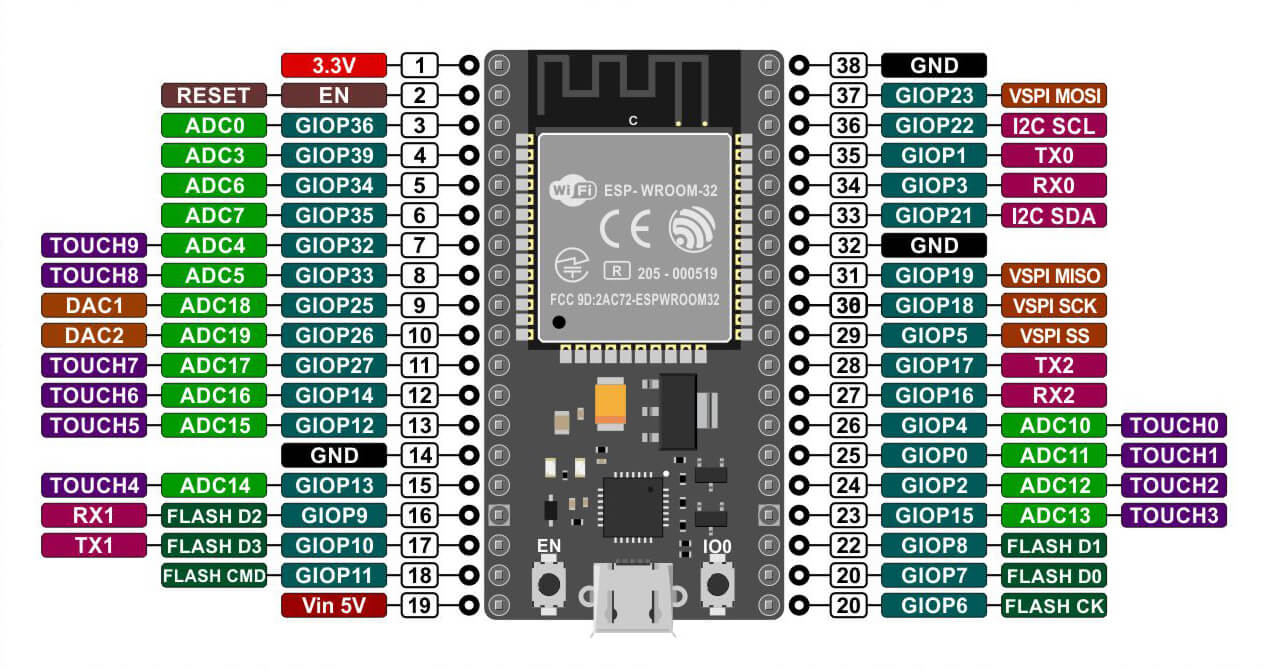
\includegraphics[width=0.8\textwidth]{figures/esp32-pinout.jpg}
    \caption{ESP32-WROOM-32E en Devkitc v4 con \textit{pinout}~\cite{esp32-pinout}.}
    \label{fig:esp32-pinout}
\end{figure}

Esta versión del \ac{SoC} dispone de un microprocesador de 32-bit Xtensa LX6 con 2 núcleos a una frecuencia máxxima de 240 MHz.
En cuanto a memoria, incluye 520 kB de memoria SRAM, 448 kB de memoria ROM y 4, 8 o 16 MB de memoria \textit{flash}.

Respecto a las comunicaciones, este dispositivo puede hacer uso del estándar 802.11 b/g/n al igual que Bluetooth v4.2 y Bluetooth LE.
Para estos estándares, incluye una antena en la parte superior, como se puede apreciar en la Figura~\ref{fig:esp32-pinout}.

Por otro lado, este dispositivo incluye una serie de periféricos como \ac{SPI}, \ac{UART}, \ac{SDIO}, \ac{I2C} y \ac{GPIO}.



\subsection{RP2040}\label{subsec:RP2040}

Por otro lado, disponemos del microcontrolador RP2040~\cite{rp2040-spec}.
Este microcontrolador se puede apreciar en varios dispositivos como Raspberry Pi Pico y Raspberry Pi Pico W.
La primera de ellas se puede apreciar en la Figura~\ref{fig:raspberry-pico}.

\begin{figure}[h]
    \centering
    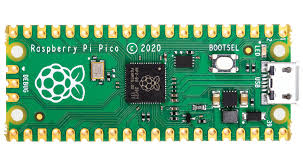
\includegraphics[width=0.6\textwidth]{figures/raspberry-pico.jpeg}
    \caption{Raspberry Pi Pico~\cite{rp2040-img}.}
    \label{fig:raspberry-pico}
\end{figure}

Este microcontrolador consta de dos procesadores ARM Cortex-M0+ a una frecuencia de 133 MHz.

En cuanto a memoria, dispone de 264 kB de SRAM en seis bancos independientes y soporta el uso de una memoria \textit{flash} de 16 MB a través de un bus QSPI.
Además, cuenta con un controlador \ac{DMA}.

En cuanto a comunicaciones, este dispositivo cuenta 2 módulos \ac{UART}, 2 controladores \ac{SPI} y 2 controladores \ac{I2C}.

En lo que respecta a periféricos, este microcontrolador dispone de 30 pines \ac{GPIO}, de los cuales 4 pueden ser utilizados como entradas analógicas.


\subsection{STM32}\label{subsec:stm32}

Por último, tenemos la familia de dispositivos STM32 basados en los procesadores ARM Cortex-M.
Esta familia está compuesta por un gran número de dispositivos.
De todos ellos, se va a proceder a explicar las características de STM32L4R5ZIT6U~\cite{nucleo-spec}.
Esto se debe a que se utilizará el dispositivo NUCLEO-L4R5ZI, el cual hace uso de microcontrolador STM32L4R5ZIT6U.
En la Figura~\ref{fig:nucleo-l4r5zi} se puede apreciar el dispositivo NUCLEO-L4R5ZI.

\begin{figure}[h]
    \centering
    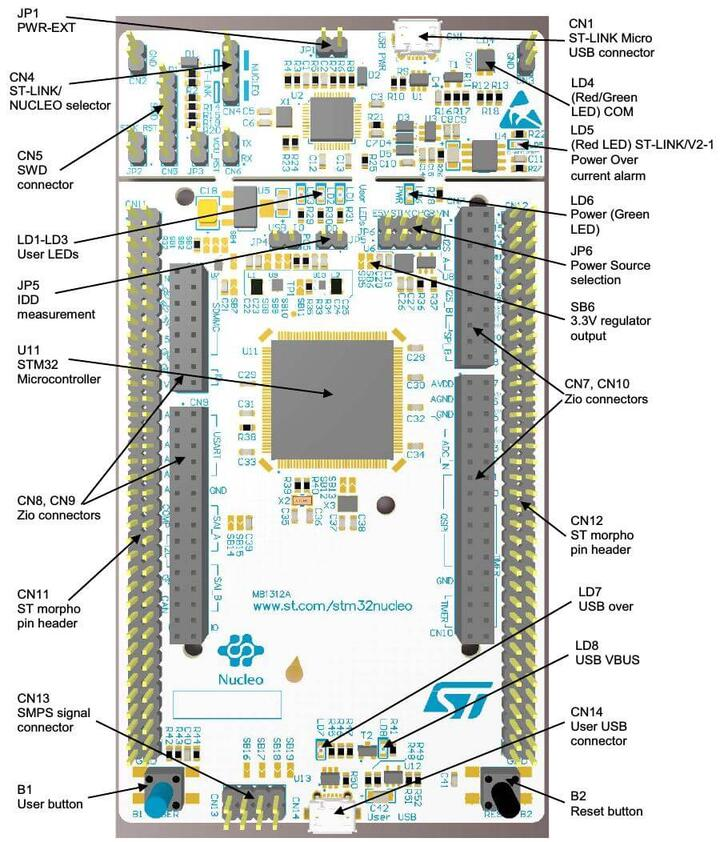
\includegraphics[width=0.6\textwidth]{figures/nucleo-l4r5zi.jpg}
    \caption{Diagrama del dispositivo NUCLEO-L4R5ZI~\cite{nucleo-img}.}
    \label{fig:nucleo-l4r5zi}
\end{figure}

El microcontrolador STM32L4R5ZIT6U consta de un procesador Arm Cortex-M4 de 32 bits con una frecuencia de hasta 120 MHz.

En lo referente a la memoria, este dispositivo dispone de una memoria \textit{flash} de 2 MB, 640 kB de memoria SRAM y una interfaz para memoria externa.
Además, dispone de un controlador \ac{DMA} con 14 canales.

Respecto a las comunicaciones, este dispositivo contiene una interfaz \ac{USB}, dos interfaces \ac{SAI}, cuatro interfaces \ac{I2C}, seis interfaces \ac{USART}, tres interfaces \ac{SPI} y un bus \ac{CAN}.



%%% Local Variables:
%%% TeX-master: "../book"
%%% End:
